\documentclass[12pt,a4paper]{article}
\usepackage{amsmath, multirow, }
\input{~/template/report/preamble.tex}
\author{ZHANGYIHENG 10.7 27}
\title{\Huge{\textbf{Investigation 6:Efficiency}} \\ \large{Physics Laboratory}}
\date{}
\begin{document}
\setmainfont{Times New Roman}
\setsansfont{Times New Roman}
\begin{spacing}{1.25}
\maketitle
\tableofcontents
\setlength{\parindent}{4ex}
\newpage
\section{Intro}
\subsection{Objective}
The investigation aims to find out the efficiency of the pulley system by analyzing the thrust required to pull the mass as well as the weight of the mass. The efficiency of the system and its tendency is deduced.
\subsection{Apparatuses}
\begin{enumerate}
    \setlength{\itemsep}{-1ex}
    \setlength{\parsep}{-1ex}
    \setlength{\topsep}{-1em}
    \item two double pulleys
    \item strong cord
    \item stand
    \item clamp
    \item meter stick
    \item weights
    \item spring balance
\end{enumerate}
\section{Procedure}
\subsection{Data Collecting}
Set up two sets of different pulley systems as the graph below shows. \par
\begin{figure}[h]
    \centering
    \subfigure[Single Pulley System]{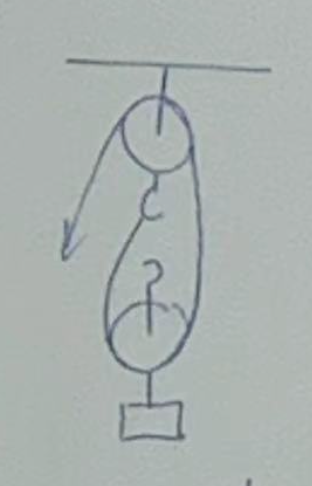
\includegraphics[width=0.45\textwidth, height = 8cm]{single.png}}
    \subfigure[Double Pulley System]{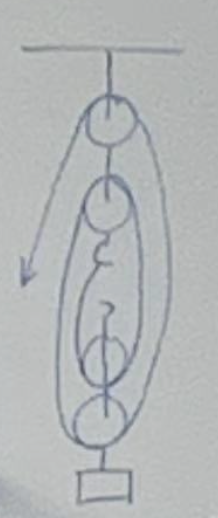
\includegraphics[width=0.45\textwidth, height = 8cm]{double.png}}
    \caption{blueprint}
    \vspace{-0.5cm}
\end{figure}
So we got the system below.
\begin{figure}[h]
    \centering
    \subfigure[Single Pulley]{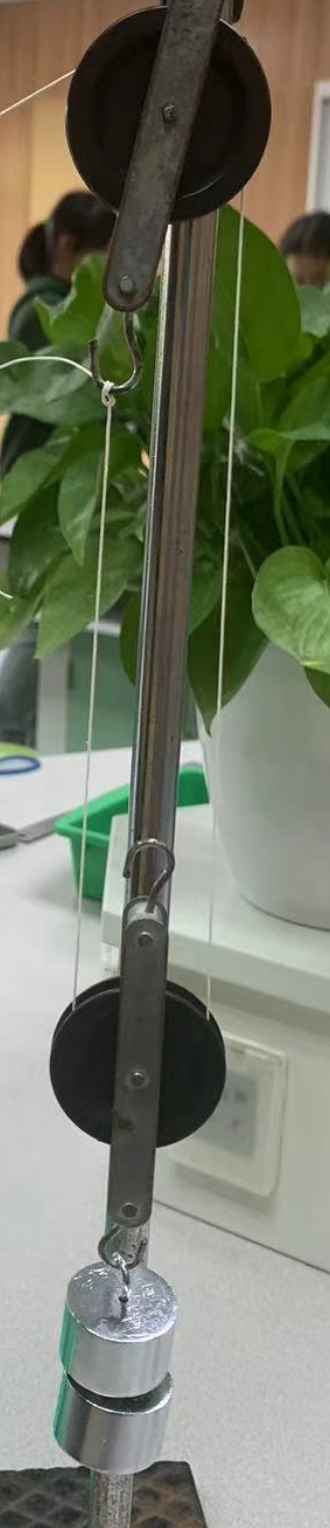
\includegraphics[width=0.25\textwidth, height = 8cm]{pulley1.png}}
    \subfigure[Double Pulley]{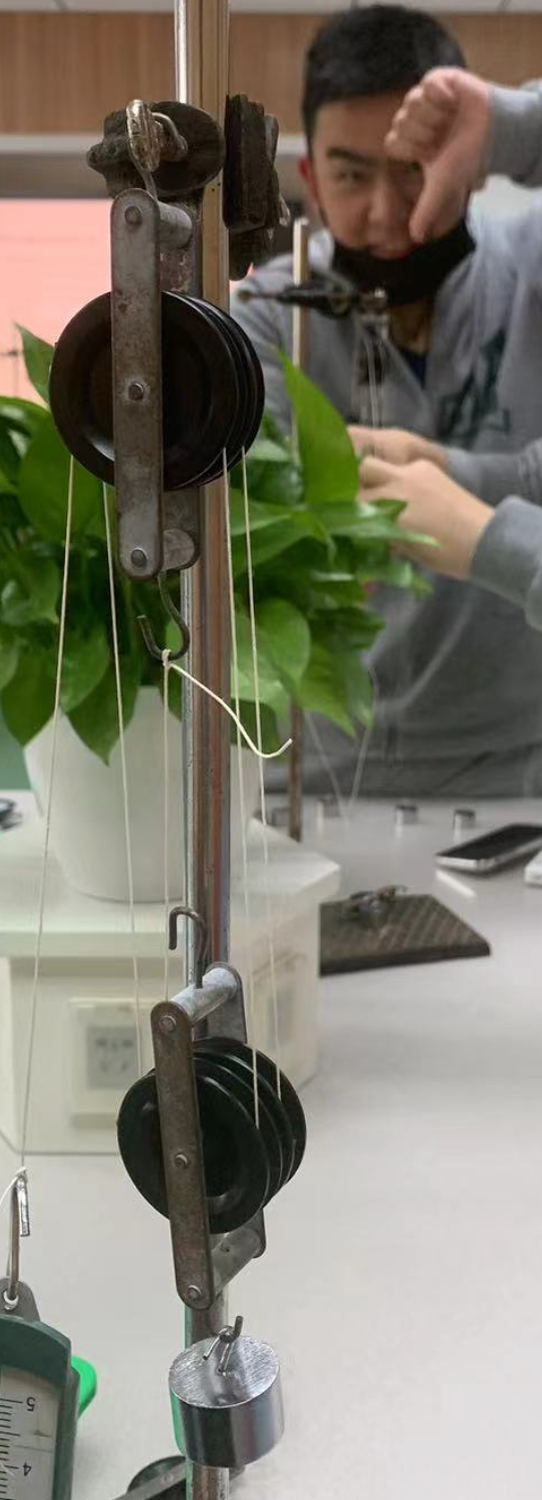
\includegraphics[width=0.25\textwidth, height = 8cm]{pulley2.png}}
    \caption{Pulley System}
    \vspace{-0.5cm}
\end{figure}\par

By reading the number of the spring dynamometer, we can obtain the thrust for pulling the weight. We changed the number of weights several times and obtained the raw data table.
\subsection{Data Processing}
Now we can use the force applied to determine the efficiency of two pulley systems. Here is one example, when there are 4 weights attached, the reading of the spring balance is 1.4 $ N $. Given the formula:\[
    \eta = \frac{W_{output}}{W_{input}} = \frac{mg\Delta h}{Fl}
\]
and $ \frac{\Delta h}{l} $ in my system is tantamount to $ \frac{1}{2} $ and $ \frac{1}{4} $ respectively.\par
So in this case, \[
    \eta = \frac{4 \times 0.05 \times 9.81}{1.4} \times \frac{1}{2} = 0.701 = 70.1\%
\]\par
Similar to the above, we can determine the $ \eta $ for all. The data obtained and recorded are in the processed data table.\par
\section{Conclusion and Evaluation}
\subsection{Conclusion}
In this experiment, by measuring the pulling force acting on the pulley, we determine the efficiency of our pulley system.\par
Taking a closer look at the relationship between efficiency and the number of masses, we can find out that $ \eta $ increases, though not significantly, with the increase of mass.
\subsection{Evaluation}
After researching on the internet, I find out we didn't consider the mass of the pulley and the friction between the string and the pulley during the investigation. This although explained our findings above. According to the formula:
\begin{align*}
    \eta  & = \frac{m_{t}g\Delta h}{Fl} \\
    & = \frac{(m_p + m_l)g \Delta h}{Fl}\\ & = \frac{(m_p + m_l)}{F} \frac{\Delta h g}{l}
\end{align*}\par
$ \frac{\Delta h g}{l} $ is a constant value and $ m_p $ remains the same on the same pulley system. Hence as $ m_l $ and $ F $ increase, the efficiency would be greater compared with the previous one.
\section{Appendix}
\begin{table}[!ht]
    \centering
    \begin{tabular}{|l|l|l|l|l|l|l|l|}
    \hline
        \multirow{3}*{Raw Data} & number of weights & 1 & 2 & 3 & 4 & 5 & 6  \\ \cline{2-8}
        ~ & system1 thrust ($ N $) & 0.4 & 0.8 & 1.1 & 1.4 & 1.7 & 2.1  \\ \cline{2-8}
        ~ & system2 thrust ($ N $) & 0.3 & 0.5 & 0.7 & 0.9 & 1.1 & 1.3  \\ \hline 
        \multirow{3}*{Processed Data} & mass($ kg $) & 0.05 & 0.1 & 0.15 & 0.2 & 0.25 & 0.3  \\ \cline{2-8}
        ~ & system1 efficiency & 0.613 & 0.613 & 0.669 & 0.701 & 0.721 & 0.701  \\ \cline{2-8}
        ~ & system2 efficiency & 0.409 & 0.491 & 0.526 & 0.545 & 0.557 & 0.566 \\ \hline
    \end{tabular}
    \caption{Data Table}
\end{table}\par
System1 refers to the pulley system with two pulleys and system2 refers to the one with four.
\begin{figure}[!htbp]
    \centering
    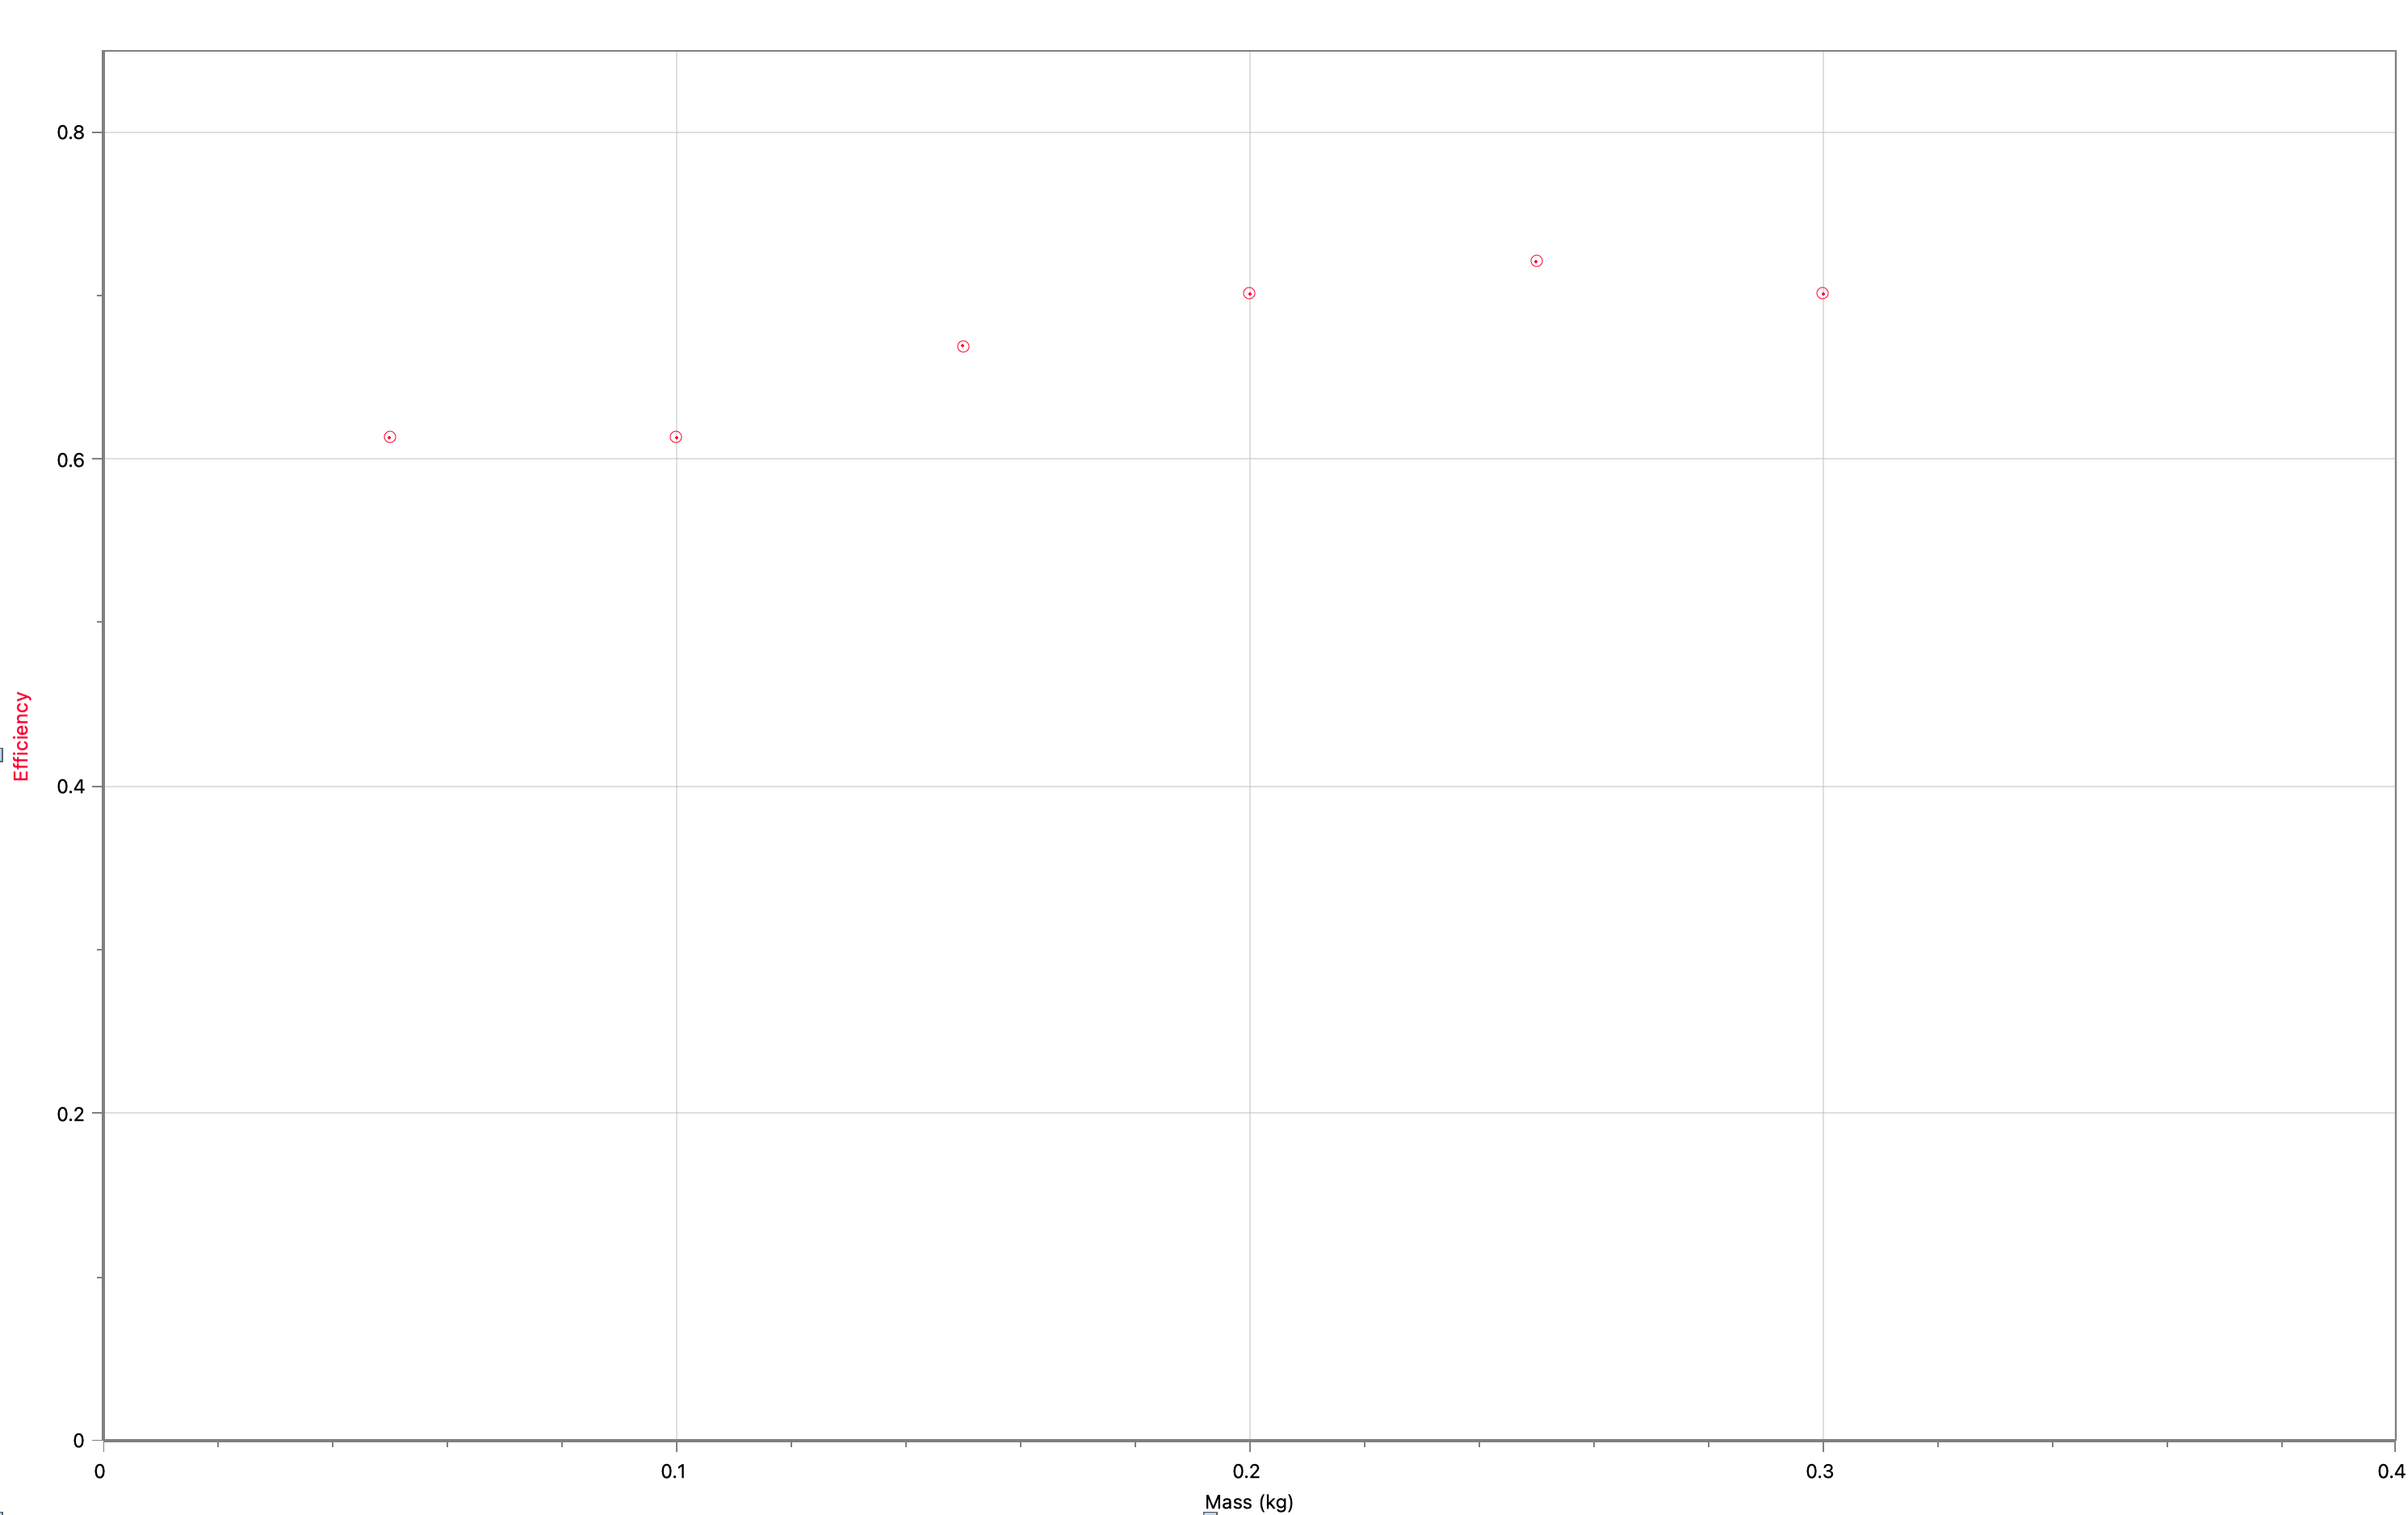
\includegraphics[width = 15cm]{graph.png}
    \caption{Efficiency against Load on Single Pulley System}
\end{figure} 

\begin{figure}[!htbp]
    \centering
    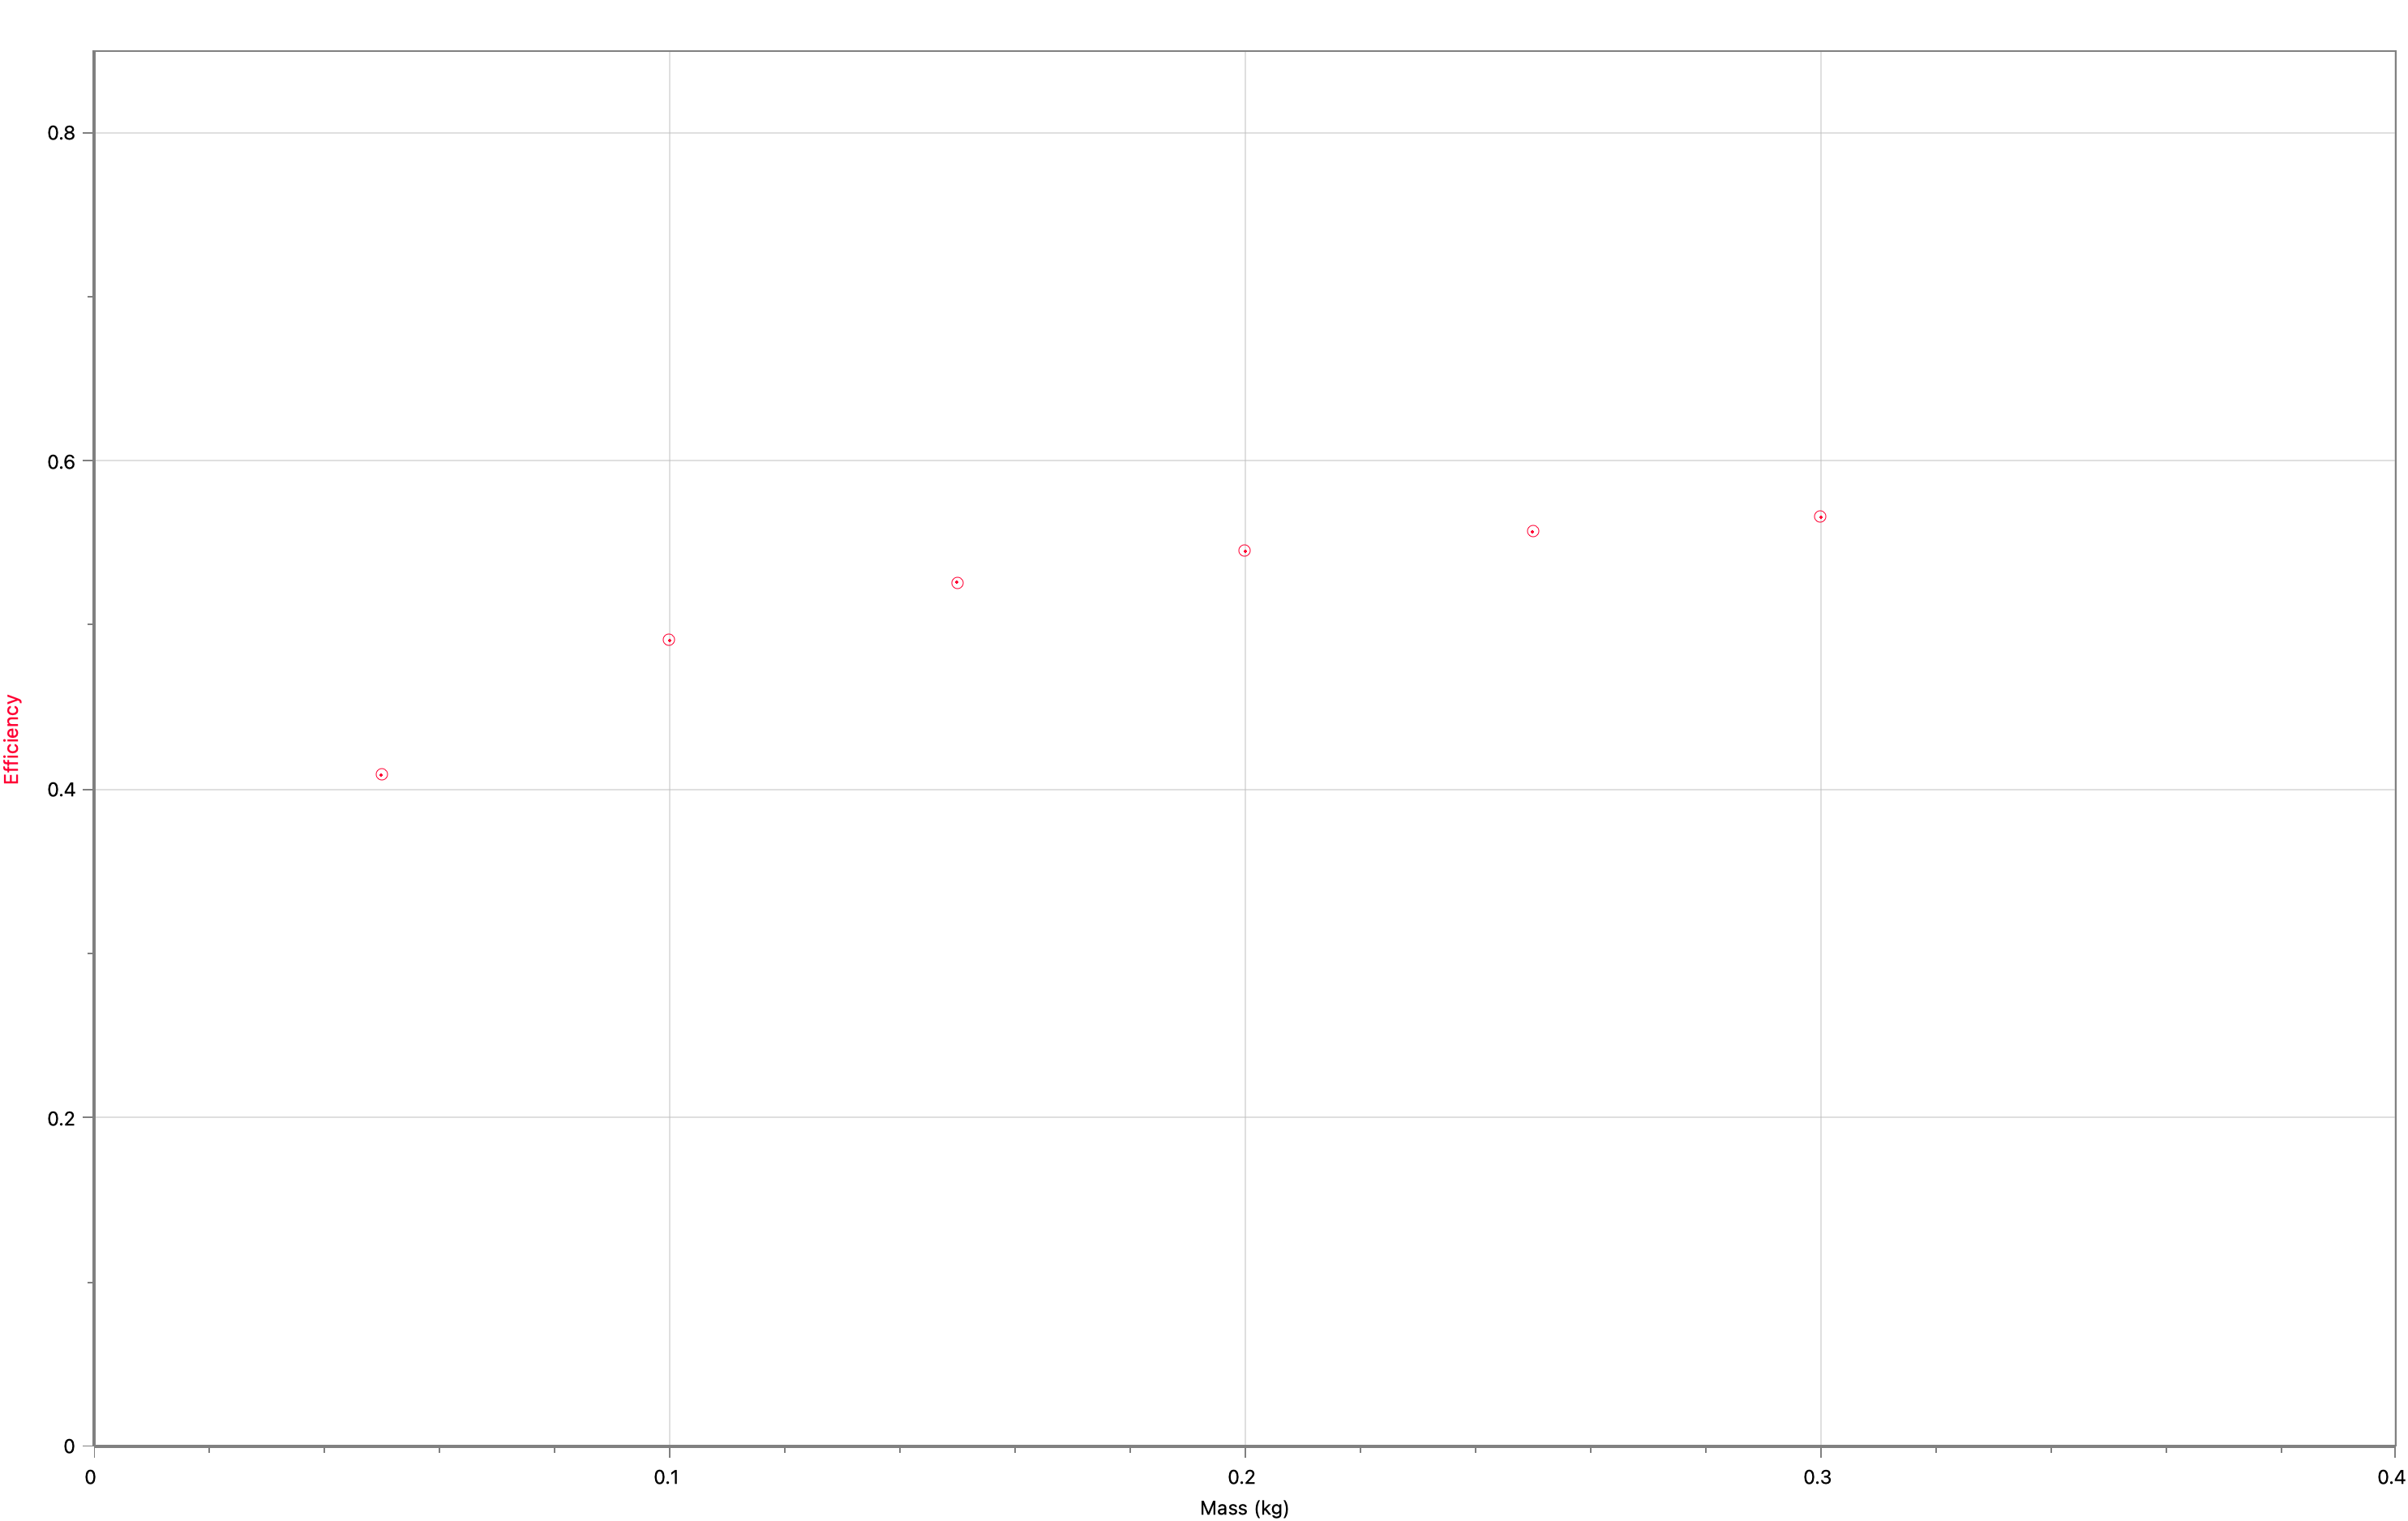
\includegraphics[width = 15cm]{graph2.png}
    \caption{Efficiency against Load on Double Pulley System}
\end{figure}
\end{spacing}

\end{document}